\documentclass{article}

\usepackage[T1]{fontenc}    %Schriftart des Dokumentes
\usepackage[ngerman]{babel} %Dokumentensprache, hier Deutsch
\usepackage{amsmath, amssymb, stmaryrd} %mathematische Schriftzeichen
\usepackage{graphicx} %Einfügen von Grafiken
\usepackage{wrapfig}
\usepackage{bm}
\usepackage{subfig}
\usepackage{newclude}
\usepackage{pdfpages}

\setlength{\parindent}{0pt} %Einrückung von Absätzen auf null gesetzt
\setlength{\parskip}{10pt} %Abstand zischen Absätzen auf 10pt gesetzt

\title{Versuch 212: Zähigkeit von Flüssigkeiten}
\author{Matthias Kuntz}
\date{23.02.2024}

\renewcommand*\contentsname{Zusammenfassung}

\begin{document}

\maketitle

\tableofcontents

\newpage

%-------------------------EINLEITUNG-------------------------
\section{Einleitung}

Untersucht man Objekte in einem Fluid oder Gas, so stellt man schnell einen gravierenden Unterschied zum Vakum fest: Wenn man möchte, dass sich das Objekt mit konstanter Geschwindigkeit bewegt, so ist eine konstante Kraft dafür nötig. Diese zunächst im Kontrast zu Newtons zweitem Gesetz scheinende Beobachtung lässt darauf schließen, dass die Medien viskos sind. In diesem Versuch soll die Viskosität von Polyethylenglykol auf zwei verschiedene Weisen untersucht werden. Zunächst werden wir fallende Kugeln im Fluid beobachten, deren Fallgeschwindigkeit nach dem Stokes'schen Gesetz abhängig von deren Radius und Dichte sowie von der Viskosität des Fluids ist. Hierbei ist auch die Beobachtung wichtig, dass fallende Objekte in einem Medium nach einer gewissen Fallzeit eine Endgeschwindigkeit erreichen, da die konstante Gravitationskraft auf diese wirkt. Des Weiteren untersuchen wir die Ausflussgeschindigkeit des Fluids, da diese über das Gesetz von Hagen-Poiseuille mit der Viskosität zusammenhängt.

\subsection{Physikalische Grundlagen}

\subsubsection{Bewegungen von und in Fluiden}

Der Grund für das bereits genannte Phänomen, dass eine konstante Kraft nötig ist um einem Körper in einem Medium eine konstante Geschwindigkeit zu geben, lässt sich darauf zurückführen, dass das Medium eine bremsende Kraft auf sich in ihm bewegende Objekte ausübt. Diese Kraft kommt von der inneren Reibung. Bei der Bewegung durch das Medium muss dieses verdrängt werden. Zudem wird von einem Objekt immer ein Teil des Mediums mitbewegt. Somit entstehen die Reibungskräfte aus den zwischenmolekularen Kräften und sind daher abhängig von der Zähigkeit des Mediums. 

\begin{figure}[!h]
    \centering
    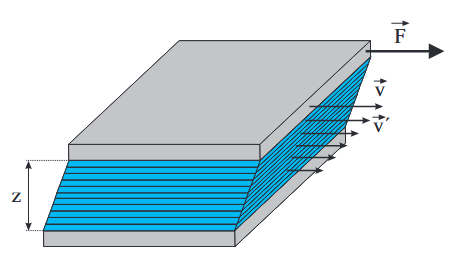
\includegraphics[width=0.6\textwidth]{graphics/gedankenexp.png}
    \caption{Gedankenexperiment zur Bestimmung der inneren Reibung [Quelle: PAP2.1 Skript, S.11, Stand: 25.02.2024]}
    \label{fig:gedankenexp}
\end{figure}

Zur Quantifizierung der Reibungskräfte in einem Medium betrachten wir das in Abbildung \ref{fig:gedankenexp} dargestellte Gedankenexperiment. Von zwei parallelen Platten, zwischen denen sich ein Fluid befindet, wird auf die obere eine parallele Kraft ausgeübt, sodass sich diese mit einer konstanten Geschwindigkeit gegenüber der ruhenden unteren Platte bewegt. Die Zähigkeit des Fluids bewirkt nun durch die Adhäsion, dass sich an beiden Platten jeweils eine Schicht des Fluids mit der exakten Geschwindigkeit der jeweiligen Platte befindet und somit sorgen die Stetigkeitsbedingungen dafür, dass die Schichten dazwischen mit unterschiedlichen, von unten nach oben zunehmenden Geschwindigkeiten aneinander vorbeigleiten. Jede Schicht beschleunigt von oben die untere und wird gleichzeitig von der untendrunter abgebremst. Die Newtonsche Reibungskraft ergibt sich hierbei zu folgender Form:

\begin{equation}
    F_r = \eta A \frac{dv}{dz}.
    \label{eq:NewtonReibung}
\end{equation}

Hierbei steht $\eta$ für die Viskosität des Mediums, $A$ für die Fläche der Platten und $\frac{dv}{dz}$ für den Geschindigkeitsgradienten zwischen den Platten. 

Grundsätzlich gibt es zwei verschiedene Arten von Strömungen: laminar und turbulent. Bei laminarer Strömung gleiten die einzelnen Flüssigkeitsschichten parallel zueinander aneinander ab ohne sich dabei zu vermischen. Das sorgt dafür, dass das Fluid einen Körper einfach symmetrisch umfließt, wie zu sehen in Abbildung \ref{fig:laminar}. Werden jedoch die Geschwindigkeiten zu groß oder die Körpergeometrien zu speziell, so treten Turbulenzen auf. Es kommt zur Bildung von Wirbeln und die Schichten beginnen sich zu vermischen, Abbildung \ref{fig:turb}. Der Strömungswiderstand ist nun viel größer und das Newtonsche Reibungsgesetz gilt nicht mehr.

\begin{figure}[!h]
  \centering
  \subfloat[Laminare Strömung]{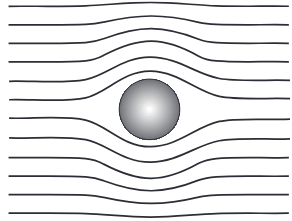
\includegraphics[width=0.45\textwidth]{graphics/laminar.png}\label{fig:laminar}}
  \hfill
  \subfloat[Turbulente Strömung]{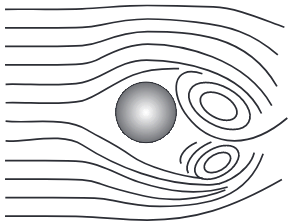
\includegraphics[width=0.45\textwidth]{graphics/turb.png}\label{fig:turb}}
  \hfill
  \caption{Bewegung einer Kugel durch ein Medium [Quelle: PAP2.1 Skript, S.11, Stand: 25.02.2024]}
  \label{fig:LaminarUndTurbulent}
\end{figure}

\subsubsection{Reynoldszahl}

Eine Abschätzung, ob sich ein Fluid laminar oder turbulent verhält, ist die sogenannte Reynoldszahl:

\begin{equation}
    Re = \frac{2 E_{kin}}{W_{Reibung}}.
    \label{eq:Reynolds}
\end{equation}

Das Verhältnis der doppelten kinetischen Energie $E_{kin}$ eines Volumenelements des Fluids zu den Reibungsverlusten $W_{Reibung}$ lässt sich dabei folgendermaßen interpretieren: Bei kleinen Reynoldszahlen, ergo für $E_{kin} \leq W_{Reibung}$, strömt das Fluid laminar und bei großen Zahlen oberhalb eines kritischen Werts $Re_{kr}$, wobei $E_{kin} \gg W_{Reibung}$ gilt, strömt es turbulent. 

Analog kann man die Reynoldszahl mit einer charakteristischen Länge $L$, die die Geometrie des Systems beschreibt, und den Parametern $v$, die mittlere Strömungsgeschwindigkeit, der Dichte $\rho$ sowie der Viskosität $\eta$ beschreiben:

\begin{equation}
    Re = \frac{\rho v L}{\eta}.
    \label{eq:Reynolds_L}
\end{equation}

Allgemein hängt die kritische Reynoldszahl vom jeweiligen System ab und ist auch keine feste Grenze. Experimentell ergeben sich beispielsweise die Werte $Re_{kr} =2300$ für die Strömung eines Fluids durch ein Rohr oder $Re_{kr} \approx 1$ für die Bewegung einer Kugel durch ein Fluid.

\subsubsection{Das Kugelfallviskosimeter}

Auf eine Kugel mir Radius $r$ und konstanter Geschwindigkeit $v$ in einem Fluid wirkt wie bereits genannt eine Reibungskraft. Diese ist über das Stokes'sche Gesetzt gegeben als:

\begin{equation}
    F_r = 6 \pi \eta r v.
    \label{eq:stokes}
\end{equation}

Da dieses Gesetzt theoretisch nur für unendlich ausgedehnte Flüssigkeiten mit laminarer Strömung gilt, wird die Ladenburg'sche Korrektur $\lambda$ im Stokes'schen Gesetz eingeführt:

\begin{equation}
    F_r = 6 \pi \eta r v \lambda \ \ \ \ \ \text{mit} \ \ \ \ \ \lambda = \left( 1 + 2,1 \cdot \frac{r}{R} \right)
    \label{eq:ladenburg}
\end{equation}

Hierbei wird das Verhältnis vom Kugelradius $r$ und dem Fallrohrradius $R$ berücksichtigt.

Somit kann man nun die Viskosität bestimmen. Auf eine Kugel im Fluid wirken insgesamt drei Kräfte: Die Reibungskraft $F_r = -6 \pi \eta r v_s$, die Auftriebskraft $F_a = - \rho_f V_k g$ sowie die Gravitationskraft $F_g = \rho_K V_k g$. Hierbei bezeichnen die Größen mit Index '$f$' das Fluid und die mit Index '$k$' die Kugel. Bewegt sich die Kugel im Fallviskosimeter nach einer kurzen Zeit mit der konstanten Sinkgeschwindigkeit $v_s$ so gilt:

\begin{equation}
    F_g + F_a + F_r = 0.
\end{equation}

Somit erhält man nach einsetzen und Auflösen nach $\eta$:

\begin{equation}
    \eta = \frac{2}{9} \ g \ \frac{(\rho_k - \rho_f)}{v_s} \ r_k^2
    \label{eq:visk_stokes}
\end{equation}

\subsubsection{Geschwindigkeit einer im Fluid fallenden Kugel}

Wir möchten nun die Geschwindigkeit einer im Fluid fallenden Kugel herleiten. Dazu machen wir den allgemeinen Ansatz mit den Kräften von oben:

\begin{equation}
    \begin{split}
        m_k a &= F_g + F_a + F_r \\
        \Rightarrow m_k \dot{v}(t) &= \rho_K V_k g - \rho_f V_k g - 6 \pi \eta r v(t) \\
        \Rightarrow \dot{v}(t) + \frac{6 \pi r_k \eta}{m_k} v(t) &= \frac{gV_k}{m_k} (\rho_k - \rho_f)  
    \end{split}
\end{equation}

Wir haben nun eine Differentialgleichung der Form $\dot{v} + \beta v = \alpha$, welche wir ganz einfach lösen können, indem wir mit dem Faktor $\exp(\beta t)$ multiplizieren und danach beide Seiten integrieren:

\begin{equation}
    \begin{split}
        \dot{v} \exp(\beta t) + \beta v \exp(\beta t) &= \alpha \exp(\beta t) \\
        \int \left[ \dot{v} \exp(\beta t) + \beta v \exp(\beta t) \right] dt &= \int \left[ \alpha \exp(\beta t) \right] dt \\
        \Rightarrow v \exp(\beta t) &= \frac{\alpha}{\beta} \exp(\beta t) + C \\
        \Rightarrow v(t) &= \frac{\alpha}{\beta} + C \exp(-\beta t)
    \end{split}
\end{equation}

Somit haben wir bereits unsere allgemeine Lösung bestimmt. Mit der Anfangsbedingung $v(0) = 0$ bestimmt sich die Konstante $C$ zu $C = - \frac{\alpha}{\beta}$ und wir können die finale Gleichung erhalten indem wir wieder $\alpha$ und $\beta$ substituieren:

\begin{equation}
    \begin{split}
        v(t) &= \frac{\alpha}{\beta} [1 - \exp(- \beta t)] \\
        v(t) &= \frac{V_k (\rho_k - \rho_f)}{6 \pi r_k \eta} \left[ 1 - \exp{\left( - \frac{6 \pi r_k \eta}{m_k} \cdot t \right)} \right]
    \end{split}
\end{equation}

Somit bestätigt sich auch, dass sich die Kugeln einer konstanten Fallgeschwindigkeit $v_s$ annähren, nachdem sie eine kurze Zeit im Medium gefallen sind. 

\subsubsection{Laminare Rohrströmung und Hagen-Poiseuille}

Der zweite Weg die Viskosität zu bestimmen ist über das Gesetz von Hagen-Poiseuille. Wir betrachten zur Herleitung ein Rohr der Länge $L$ und Radius $R$, durch das eine Flüssigkeit strömt. Damit es zur Strömung kommt, muss an den beiden Stirnflächen des Rohrs eine Druckdifferenz $\Delta p = p_1 - p_2$ herrschen. Wir betrachten wieder einen laminaren Fluss mit Schichtströmung. Die Kraft aufgrund der Druckdifferenz auf einen koaxialen Teilzylinder mit Radius $r<R$ im Rohr ergibt sich zu

\begin{equation}
    F_p = \pi r^2 (p_1 - p_2).
\end{equation}

Zudem wirkt wieder die Newtonsche Reibungskraft $F_r = - 2 \pi r L \eta \frac{dv}{dr}$. Für einen konstanten Strom muss nun $F_p + F_r = 0$ gelten, woraus man den Geschwindigkeitsgradienten erhält:

\begin{equation}
    \frac{dv}{dr} = \frac{(p_1 - p_2)}{2 \eta L} r.
\end{equation}

Daraus lässt sich die Geschwindigkeitsverteilung in der Flüssigkeit bestimmen, indem man über $r$ integriert und die Randbedingung $v(R) = 0$ berücksichtigt:

\begin{equation}
    v(r) = \frac{(p_1 - p_2)}{4 \eta L} (R^2 - r^2).
\end{equation}

Zuletzt integrieren wir über die Querschnittsfläche des Zylinders und erhalten das Gesetzt von Hagen-Poiseuille für den Volumenstrom:

\begin{equation}
    \frac{dV}{dt} = \int_0^R 2 \pi r v(r) dr = \frac{\pi (p_1 - p_2) R^4}{8 \eta L}
    \label{eq:HagPois}
\end{equation}

Somit zeigt sich, dass man die Viskosität bestimmen kann, wenn man den Volumenstrom misst und die Parameter des Rohrs kennt.

\subsection{Versuchsaufbau}

Der Versuchsaufbau besteht aus einem langen vertikalen Rohr mit Messkala, welches mit Polyethylenglykol befüllt ist. Unten am Rohr ist eine Präzisionskapillare angebracht. Zur Verfügung stehen Kugeln aus Polyacetal verschiedener Größen, sowie Pinzetten, ein Thermometer und Stoppuhren. Für den zweiten Versuchsteil ist noch ein Becherglas mit Messkala gegeben. 

\phantom{.}

\begin{figure} [!h]
    \centering
    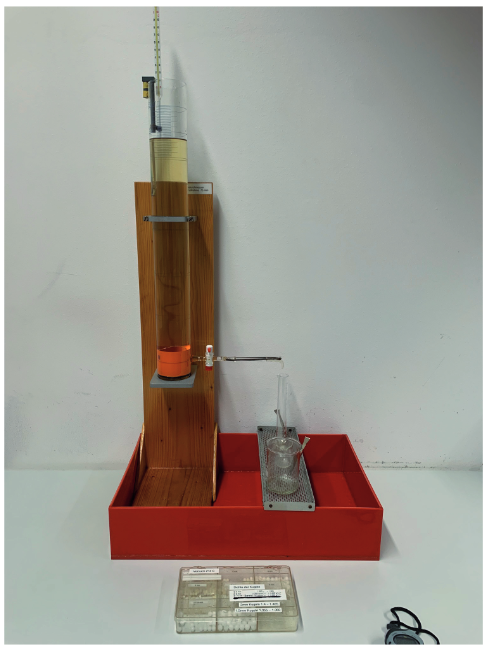
\includegraphics[height=9cm]{graphics/aufbau.png}
    \caption{Versuchsaufbau [Quelle: PAP2.1 Skript, S.11, Stand: 25.02.2024]}
\end{figure}

%---------------VERSUCHSPROTOKOLL MIT MESSDATEN---------------
\newpage

\section{Versuchsprotokoll mit Messdaten}

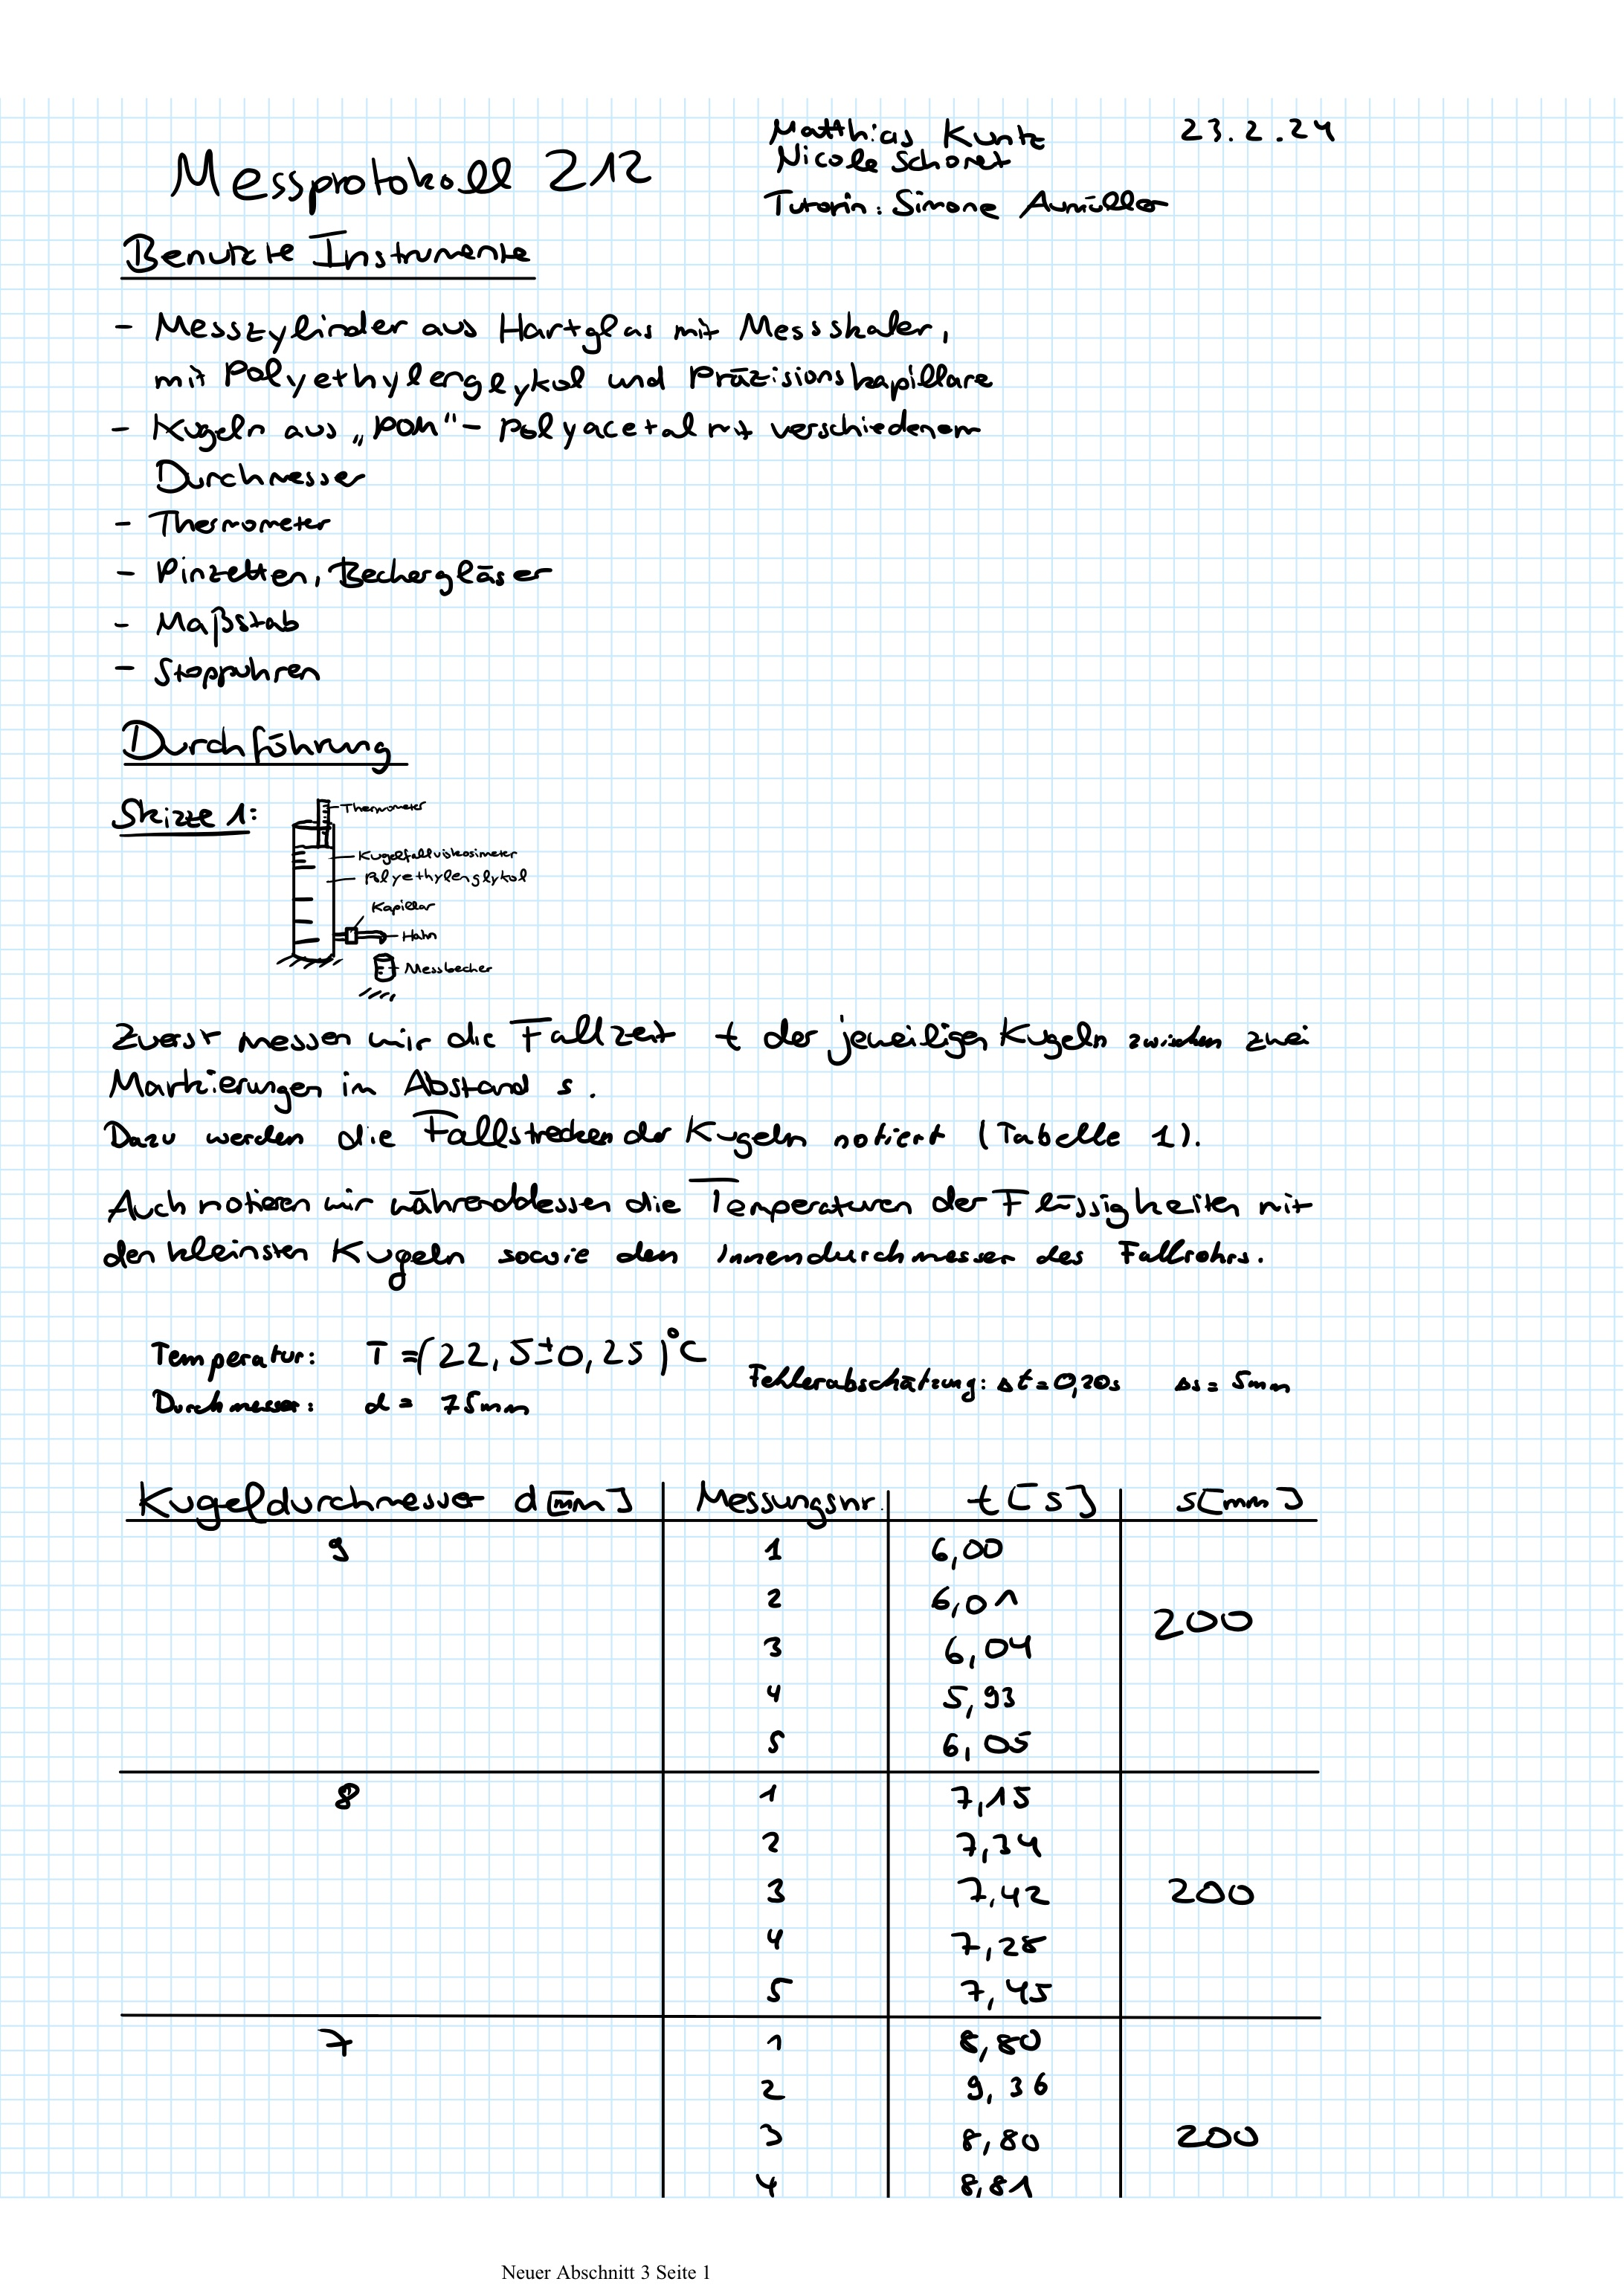
\includegraphics[width=\textwidth]{graphics/mess1.jpg}
\newpage
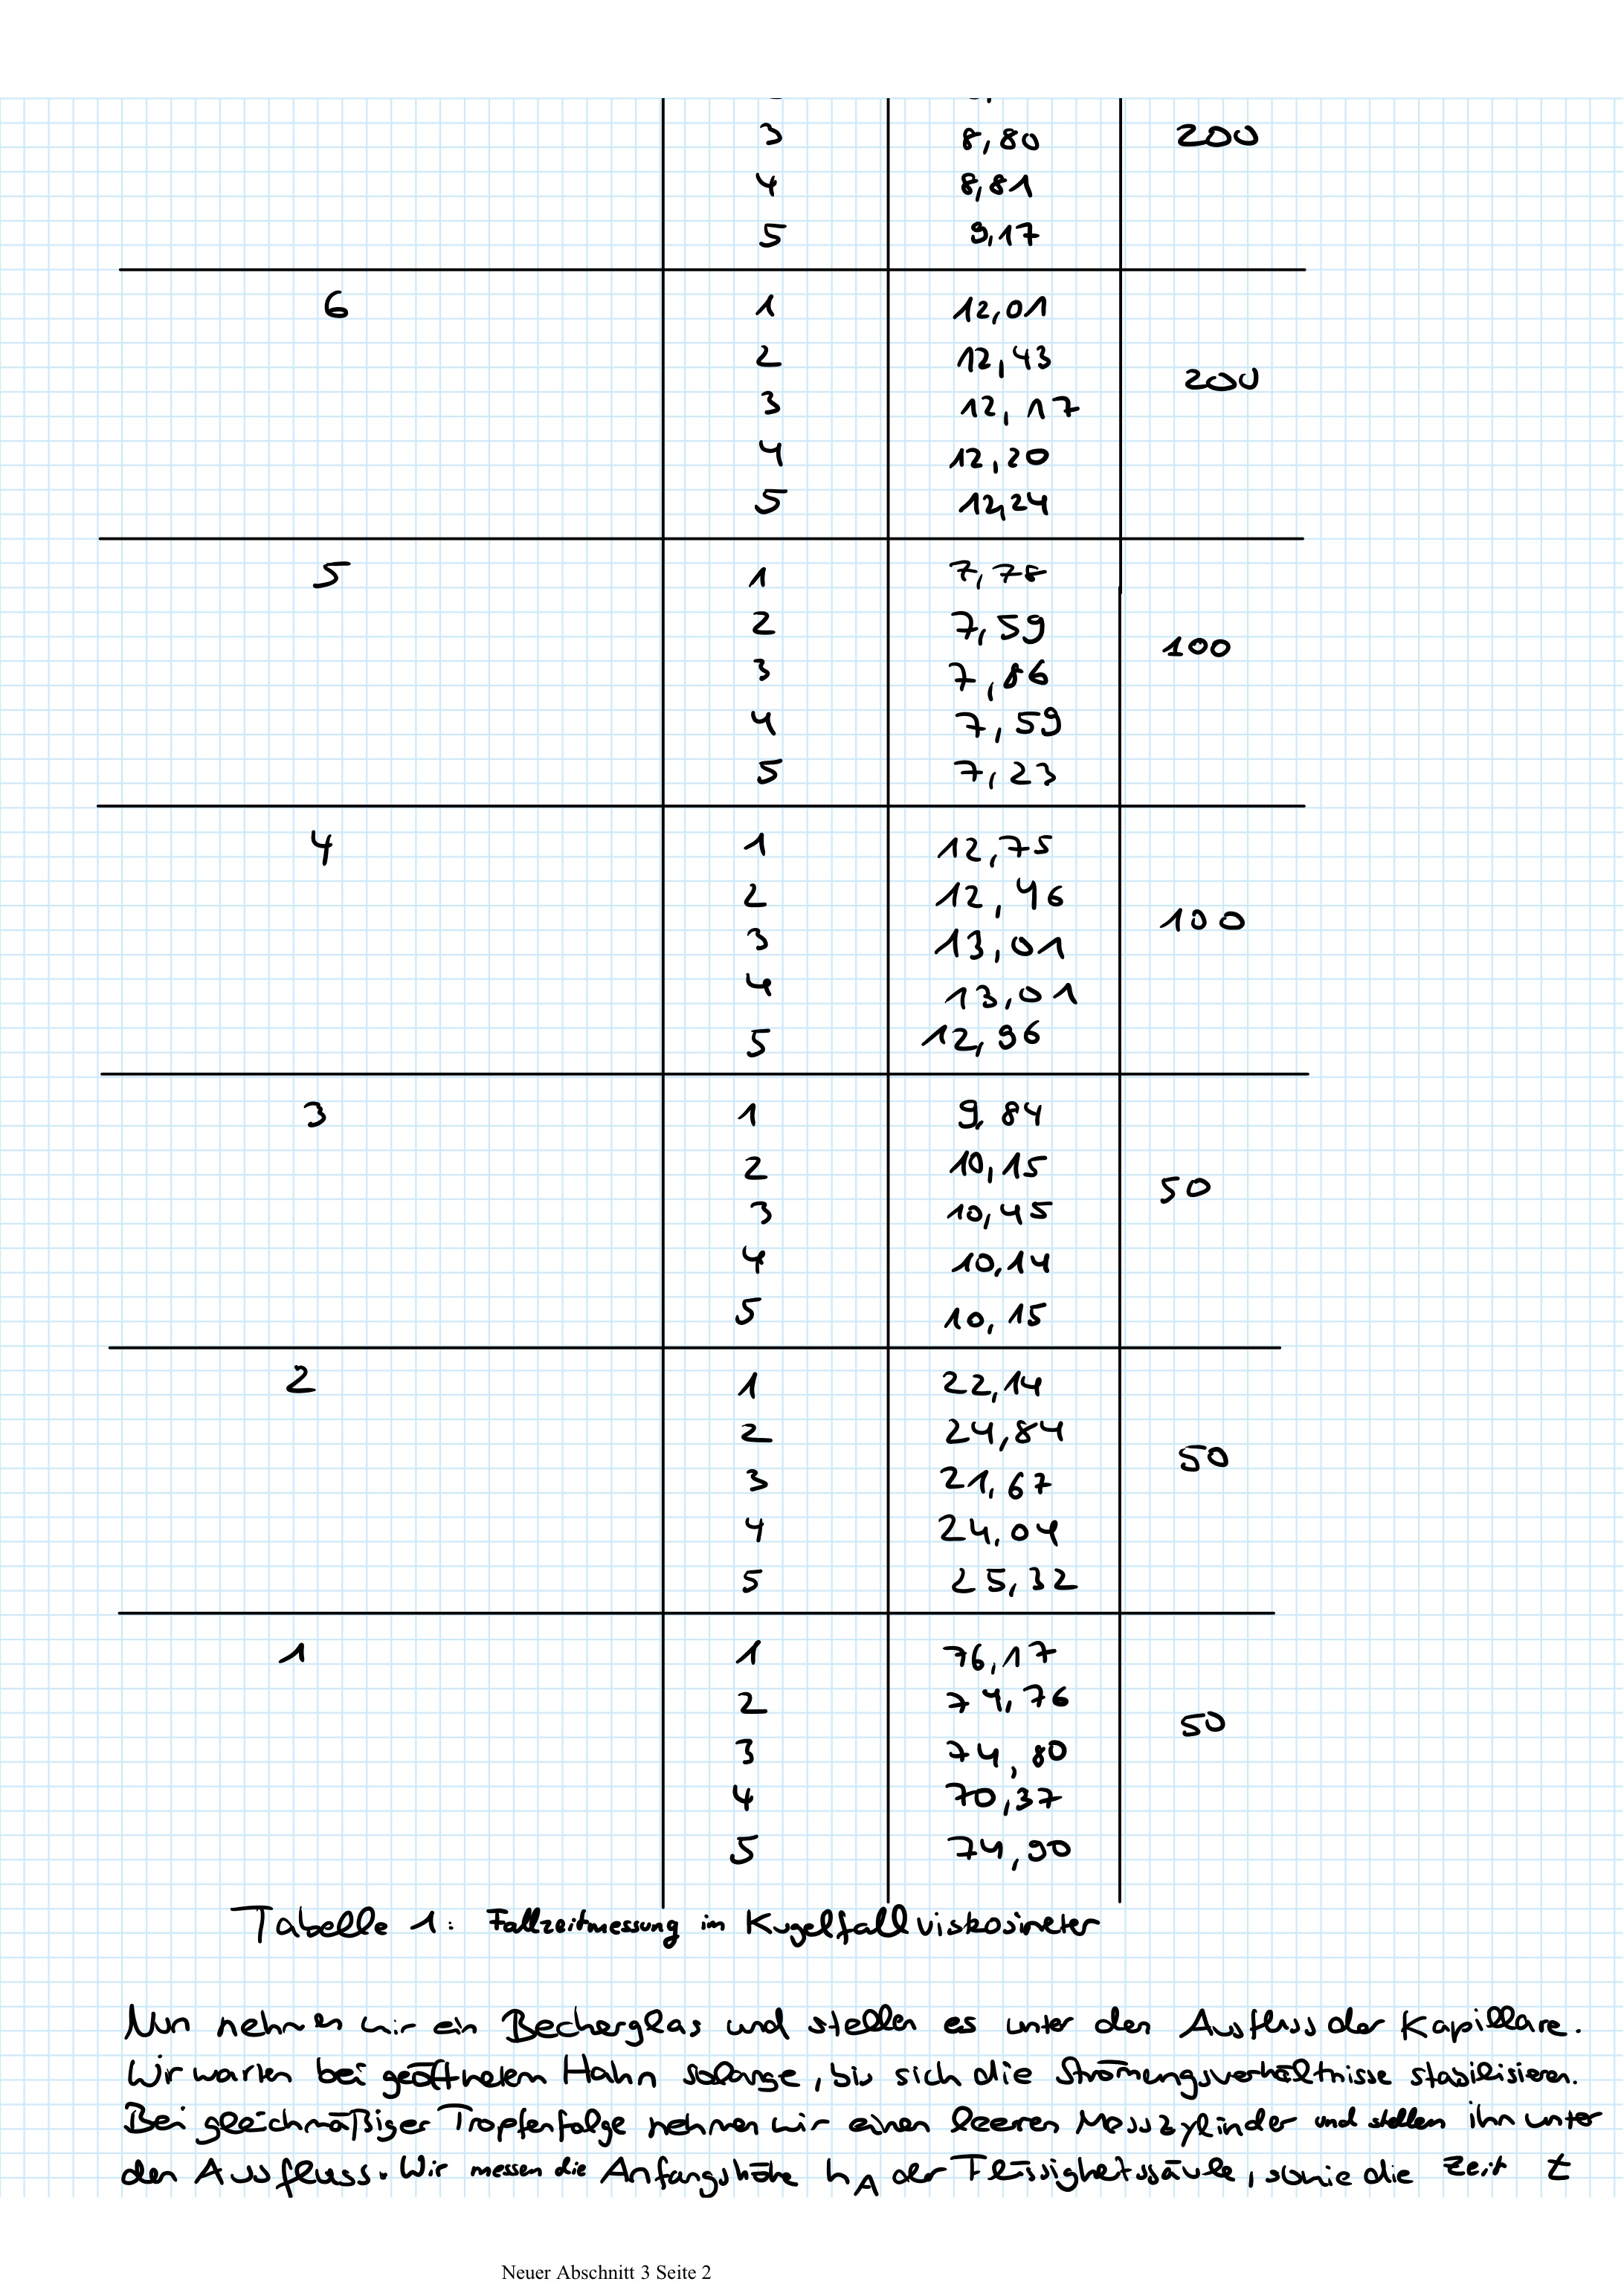
\includegraphics[width=\textwidth]{graphics/mess2.jpg}
\newpage
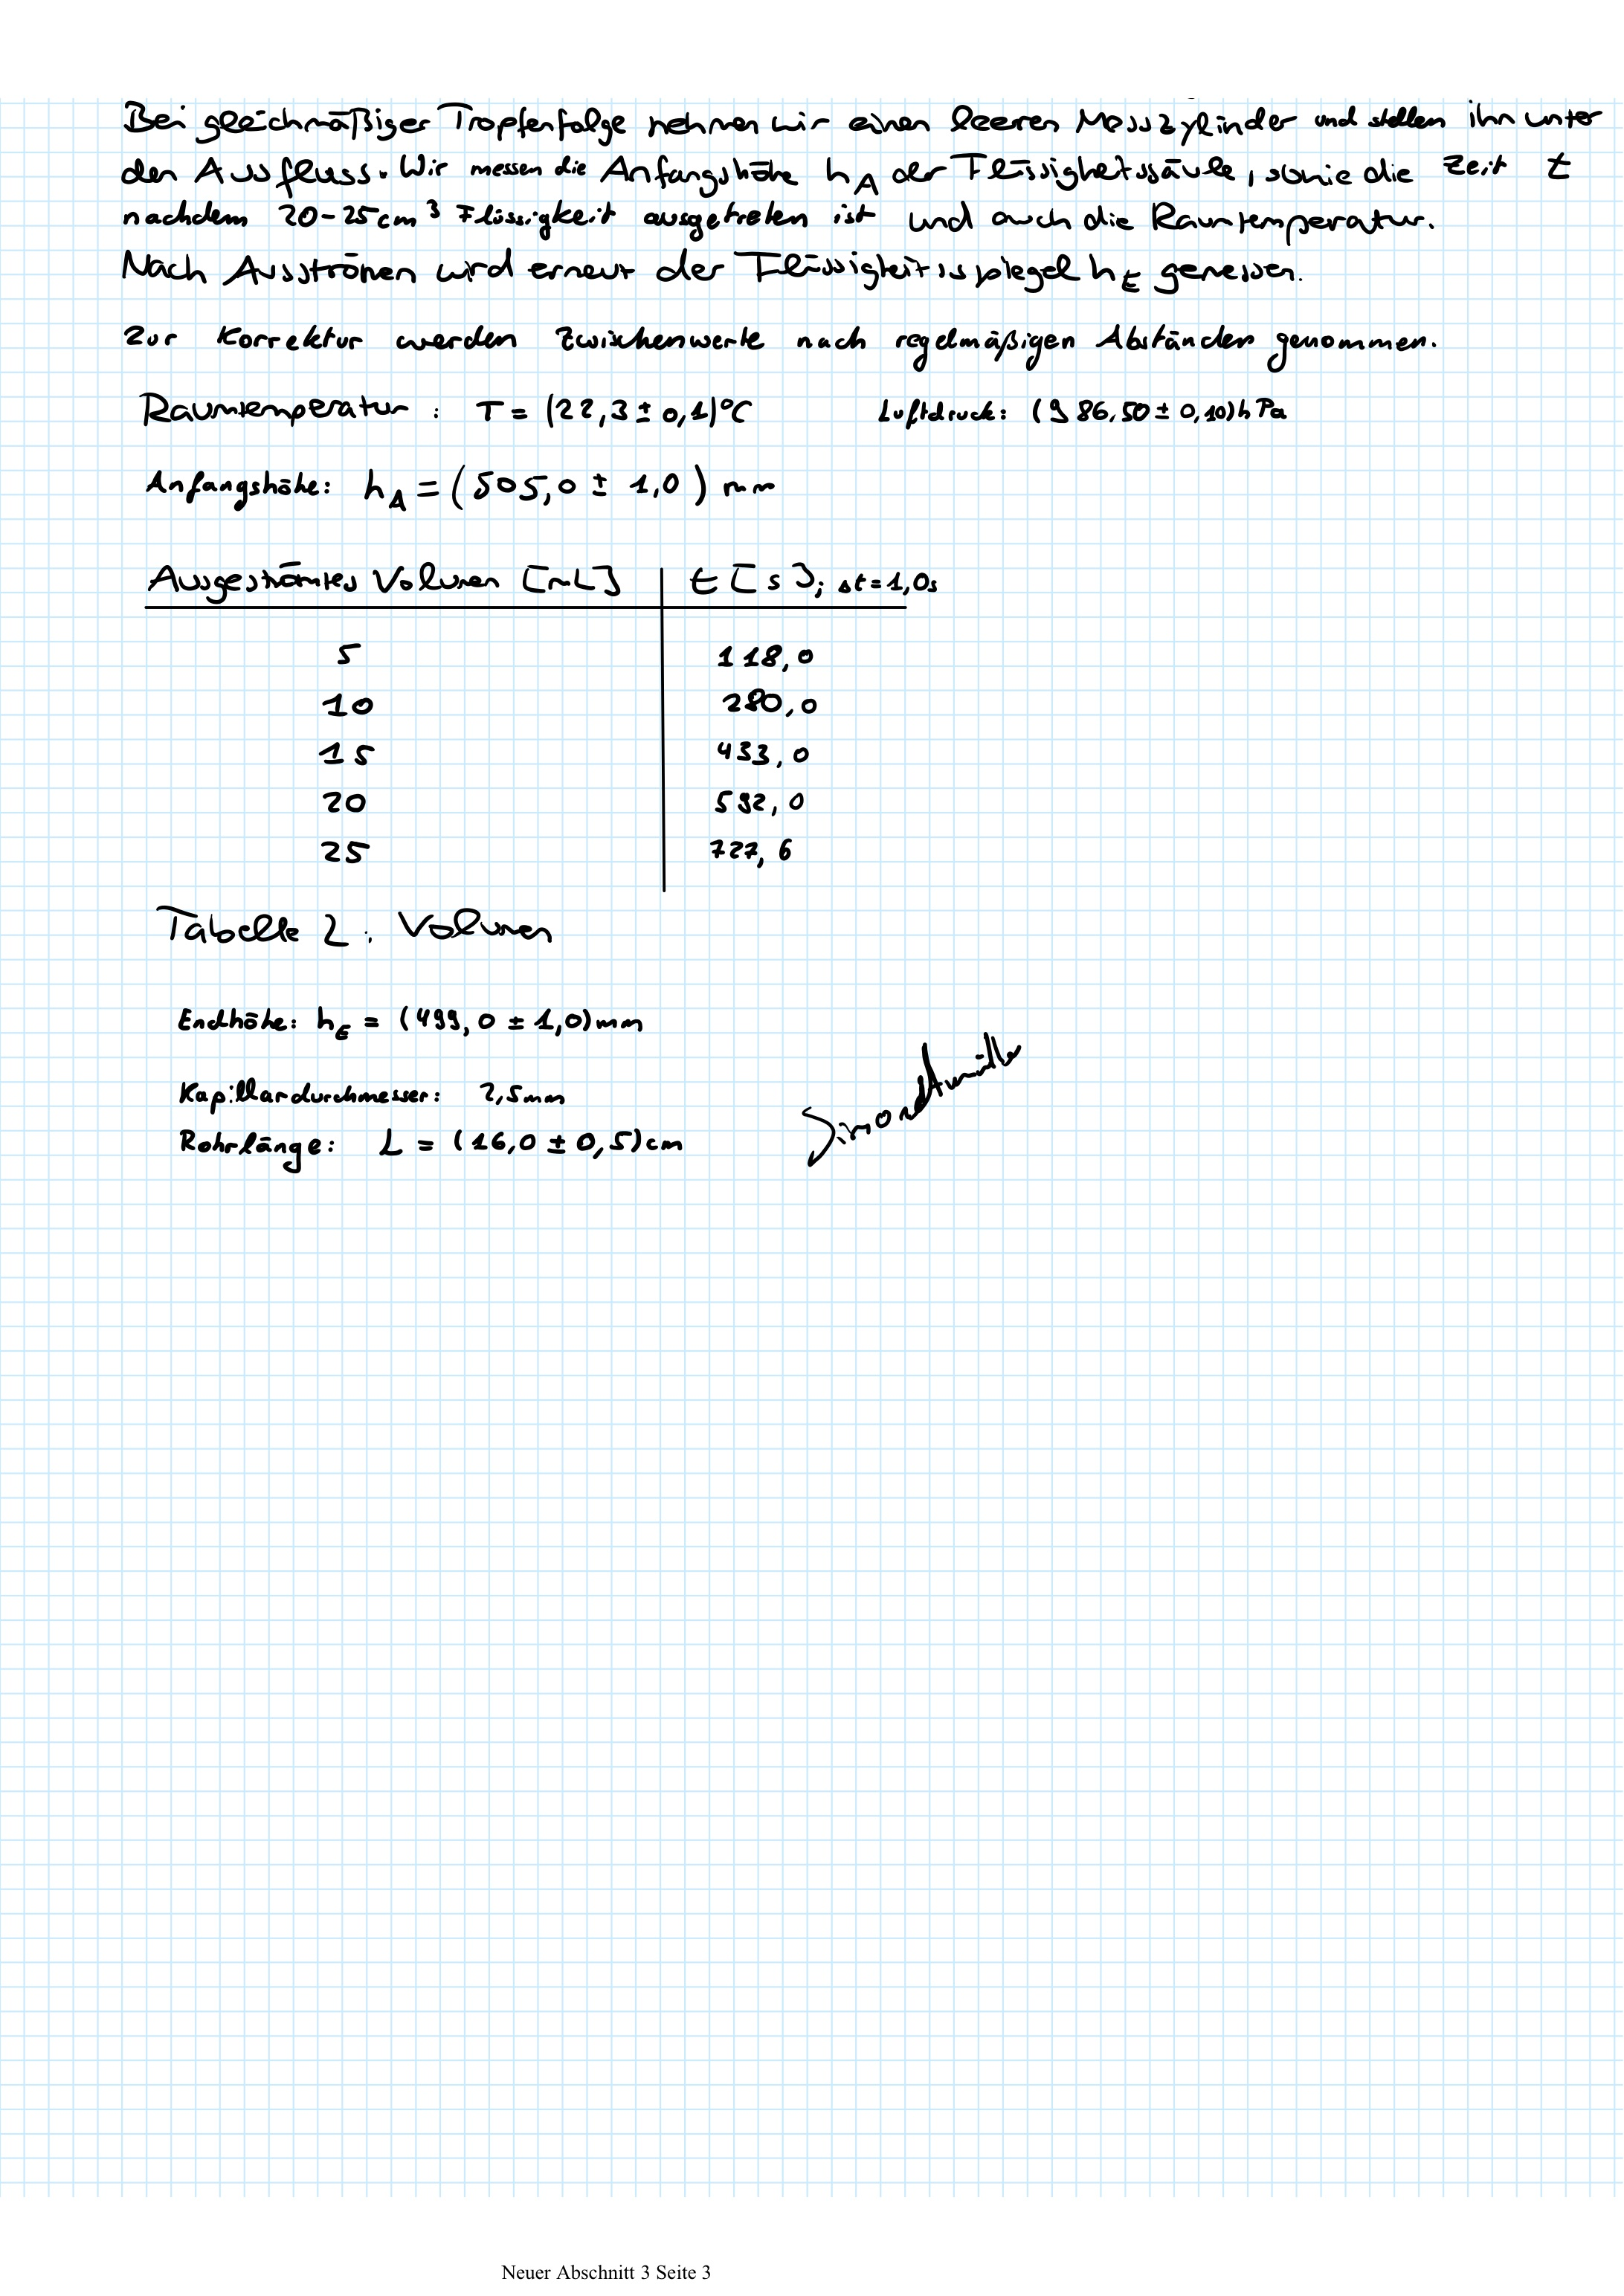
\includegraphics[width=\textwidth]{graphics/mess3.jpg}
\newpage

\addtocounter{table}{2}

\newpage
%-------------------------AUSWERTUNG-------------------------
\section{Auswertung}

In dieser Evaluation werden alle Fehler, sofern keine spezifische Angabe gemacht wird, mithilfe der Gauss'schen Fehlerfortpflanzung berechnet. Dies bedeutet, dass ein Wert $F$, der mit der Formel $f(a_1, ..., a_n)$ berechnet wird, den Fehler $\Delta F$ annimmt:

\begin{equation}
    \Delta F = \sqrt{\sum_n \left( \frac{\partial f}{\partial a_n} \cdot \Delta a_n \right)^2}.
\end{equation}

Des Weiteren erfolgen Signifikanztests von zwei Werten $a$ und $a'$ über die folgende Formel:

\begin{equation}
    \sigma = \frac{|a-a'|}{\sqrt{(\Delta a)^2 + (\Delta a')^2}}.
\end{equation}

Die Güte eines Fits wird mit der $\chi^2$-Summe bewertet:

\begin{equation}
    \chi^2 = \sum_i^N \left( \frac{\textit{Funktionswert}_i - \textit{Messwert}_i}{\textit{Fehler}_i} \right)^2
\end{equation}

Auch verwendet wird $\chi^2_{red} = \chi^2 / f$, wobei der Freiheitsgrad $f$ die Anzahl der Messwerte minus die Anzahl der Fitparameter ist. Der auf die Freiheitsgrade normierte Wert soll bei einem guten Fit ungefähr 1 sein.

\newpage

\subsection{Bestimmung der Viskosität nach Stokes}

Wir beginnen, indem wir die von uns gemessenen Fallzeiten auswerten. Dazu bilden wir aus den in Tabelle 1 des Messprotokolls aufgezeichneten Zeiten den Mittelwert für jede Kugelgröße. Der Fehler der Mittelwerte $\Delta t_{mean}$ setzt sich hierbei aus dem Messfehler $\Delta t = 0,20$s sowie dem Standartfehler des Mittelwerts $\sigma_{std}$ zusammen:

\begin{equation}
    \Delta t_{mean} = \sqrt{(\Delta t)^2 + (\sigma_{std})^2}.
\end{equation}

Mit den so erhaltenen Zeiten berechnen wir die durchschnittlichen Fallgeschwindigkeiten der Kugeln mit $v = s/t$. Wir verwenden die jeweiligen Fallstrecken $s$ der Tabelle 1 des Messprotokolls und der Fehler beläuft sich somit auf:

\begin{equation}
    \Delta v = v \sqrt{\left( \frac{\Delta t}{t} \right)^2 + \left( \frac{\Delta s}{s} \right)^2}.
\end{equation}

Wir tragen diese Ergebnisse zusammen mit sowohl dem Radius, als auch dem Radius zum Quadrat in Tabelle \ref{tab:t_mean&v} ein. Der Fehler des Radius wurde dem Skript entnommen, wo eine Abweichung von $\pm 25 \mu$m für die Durchmesser gegeben ist.

\phantom{.}

\begin{table}[!h]
    \centering
    %\resizebox{\textwidth}{!}{
    \begin{tabular}{cccc}
        \hline
        $\bm{r}$ [mm] & $\bm{r^2}$ [mm$^2$] & $\bm{t_{mean}}$ [s] & $\bm{v}$ [mm/s]  \\ \hline
        $0,500 \pm  0,013$   & $0,250 \pm  0,013$ & $74,2 \pm 2,0$  & $0,67 \pm 0,07$    \\
        $1,000 \pm  0,013$   & $1,000 \pm 0,025$ & $23,6 \pm 1,5$   & $2,12 \pm 0,25$    \\
        $1,500 \pm  0,013$   & $2,25 \pm 0,04$   & $10,15 \pm 0,28$ & $4,9 \pm 0,5$    \\
        $2,000 \pm  0,013$   & $4,00  \pm 0,05$  & $12,84 \pm 0,29$ & $7,8 \pm 0,4$    \\
        $2,500 \pm  0,013$   & $6,25  \pm 0,06$  & $7,6 \pm 0,3$    & $13,1 \pm 0,8$    \\
        $3,000 \pm  0,013$   & $9,00  \pm 0,08$  & $12,21 \pm 0,24$ & $16,4 \pm 0,5$    \\
        $3,500 \pm  0,013$   & $12,25  \pm 0,09$ & $9,0 \pm 0,3$    & $22,3 \pm 0,9$    \\
        $4,000 \pm  0,013$   & $16,00  \pm 0,10$ & $7,33 \pm 0,23$  & $27,3 \pm 1,1$    \\
        $4,500 \pm  0,013$   & $20,25  \pm 0,11$ & $6,01 \pm 0,20$  & $33,3 \pm 1,4$    \\ \hline
    \end{tabular}%}
    \caption{Fallzeiten und Fallgeschwindigkeiten}
    \label{tab:t_mean&v}
\end{table}

\phantom{.}

Wir tragen nun die Geschwindigkeiten gegenüber dem Radius-Quadrat in ein Diagramm ein, zu sehen in Abbildung \ref{fig:v_gegen_r^2}. Da bei den eben berechneten Werten beim Plot eine klare Abweichung nach unten zum erwarteten linearen Verlauf bei größeren Werten zu sehen ist, berechnen wir direkt die Ladenburg'sche Korrektur nach Gleichung \ref{eq:ladenburg}, indem wir den Faktor $\lambda$ an unsere Geschwindigkeiten multiplizieren. Der Fehler ergibt sich somit zu:

\begin{equation}
    \Delta v_{korr} = \sqrt{\left( \Delta v  \left( 1 + 2,1 \frac{r}{R} \right) \right)^2 + \left( 2,1 v \frac{\Delta r}{R}  \right)^2}
\end{equation}


Die Ergebnisse für die korrigierten Geschwindigkeiten $v_{korr}$ sind in Tabelle \ref{tab:v_korr} notiert und werden auch im Diagramm in Abbildung \ref{fig:v_gegen_r^2} eingetragen.

\phantom{.}

\begin{table}[!h]
    \centering
    %\resizebox{\textwidth}{!}{
    \begin{tabular}{cc}
        \hline
        $\bm{r^2}$ [mm$^2$] & $\bm{v_{korr}}$ [mm/s]  \\ \hline
        $0,250 \pm  0,013$ & $0,69 \pm 0,07$     \\
        $1,000 \pm 0,025$ & $2,24 \pm 0,26$     \\
        $2,25 \pm 0,04$   & $5,3 \pm 0,6$     \\
        $4,00  \pm 0,05$  & $8,7 \pm 0,5$     \\
        $6,25  \pm 0,06$  & $15,0 \pm 0,9$     \\
        $9,00  \pm 0,08$  & $19,1 \pm 0,6$     \\
        $12,25  \pm 0,09$ & $26,6 \pm 1,1$     \\
        $16,00  \pm 0,10$ & $33,4 \pm 1,3$     \\
        $20,25  \pm 0,11$ & $41,7 \pm 1,8$     \\ \hline
    \end{tabular}%}
    \caption{Korrigierte Fallgeschwindigkeiten}
    \label{tab:v_korr}
\end{table}

\phantom{.}

\begin{figure}[!h]
    \centering
    \resizebox{0.9\textwidth}{!}{
    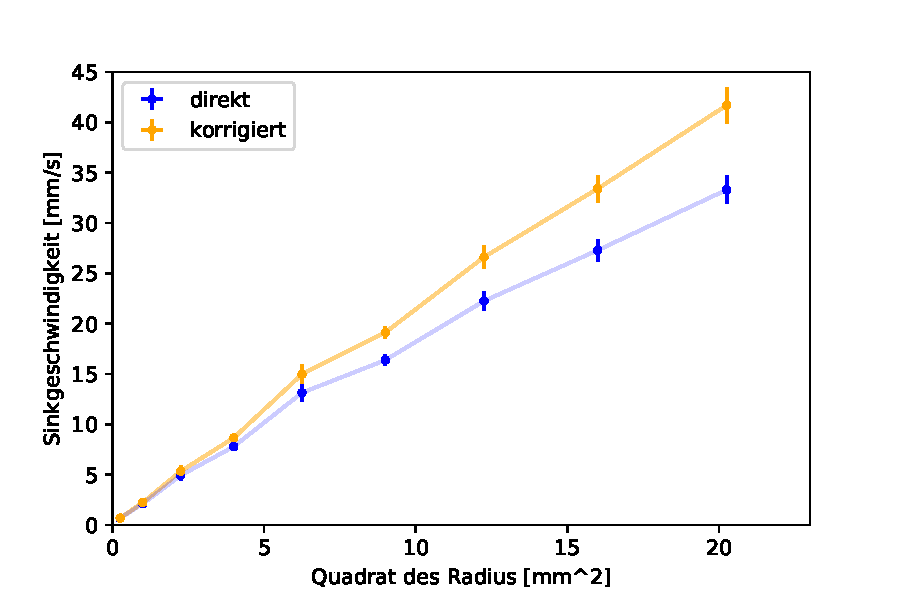
\includegraphics{graphics/plots/Geschwindigkeiten_korrektur.pdf}}
    \caption{Geschwindigkeiten gegen Radiusquadrat}
    \label{fig:v_gegen_r^2}
\end{figure}

\newpage
Wie in Abbildung \ref{fig:v_gegen_r^2} zu erkennen ist, knicken auch die korrigierten Messwerte nach dem fünften Wert nach unten ab. Dies ist der Punkt, an dem die Kugeln so groß und schnell werden, dass die Strömung nicht mehr laminar, sondern auch turbulent wird. Wir separieren also den linearen Teil, ergo die ersten fünf Werte der korrigierten Geschwindigkeiten, und fitten eine lineare Funktion an diese, um mithilfe von Gleichung \ref{eq:visk_stokes} die Viskosität aus dem Gradienten der Funktion zu berechnen. Unser Fit, zu sehen in Abbildung \ref{fig:FitStokes}, bestimmt den Gradienten $\gamma$ als:

\begin{equation}
    \gamma = (2,23 \pm 0,07) \frac{1}{\text{mm} \cdot \text{s}}
\end{equation}

\phantom{.}

\begin{figure}[!h]
    \centering
    \resizebox{0.9\textwidth}{!}{
    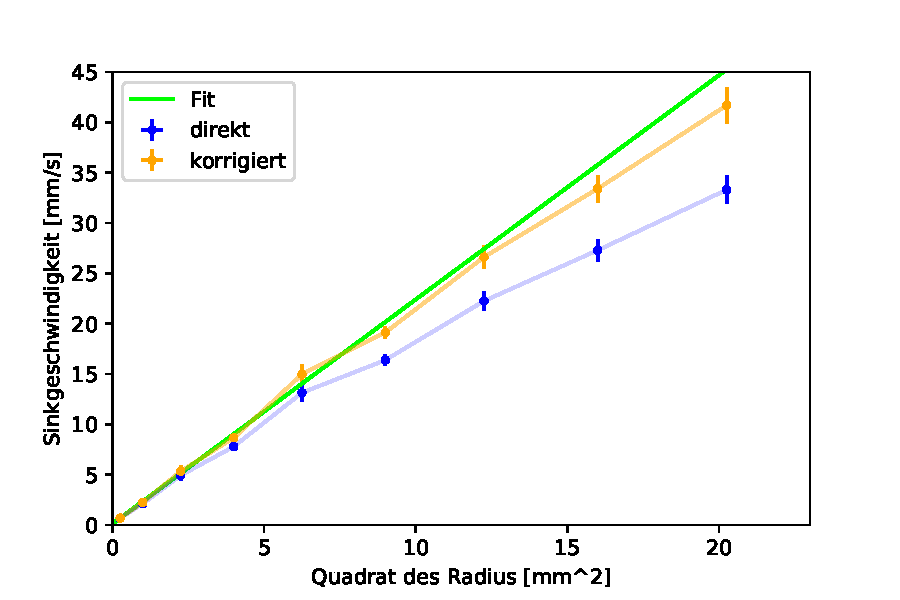
\includegraphics{graphics/plots/Fit_Stokes.pdf}}
    \caption{Linearer Fit an die korrigierten Geschwindigkeiten}
    \label{fig:FitStokes}
\end{figure}

\phantom{.}

Für die Berechnung der Viskosität benötigen wir noch die Dichten von den Kugeln und der Flüssigkeit. Die der Kugeln ist im Skript gegeben als $\rho_k = (1385 \pm 15)$kg/m$^3$ und für die der Flüssigkeit verwenden wir das dem Skript angehängte Diagramm und lesen die Dichte mithilfe der von uns gemessenen Flüssigkeitstemperatur von $(22,50 \pm 0,25)^\circ$C ab, zu sehen in Abbildung \ref{fig:Dichte_f}. Wir bestimmen somit den Wert:
\begin{equation}
    \rho_f = (1147,1 \pm 0,3) \frac{\text{kg}}{\text{m}^3}.    
\end{equation}

\begin{figure}[!h]
    \centering
    \resizebox{0.9\textwidth}{!}{
    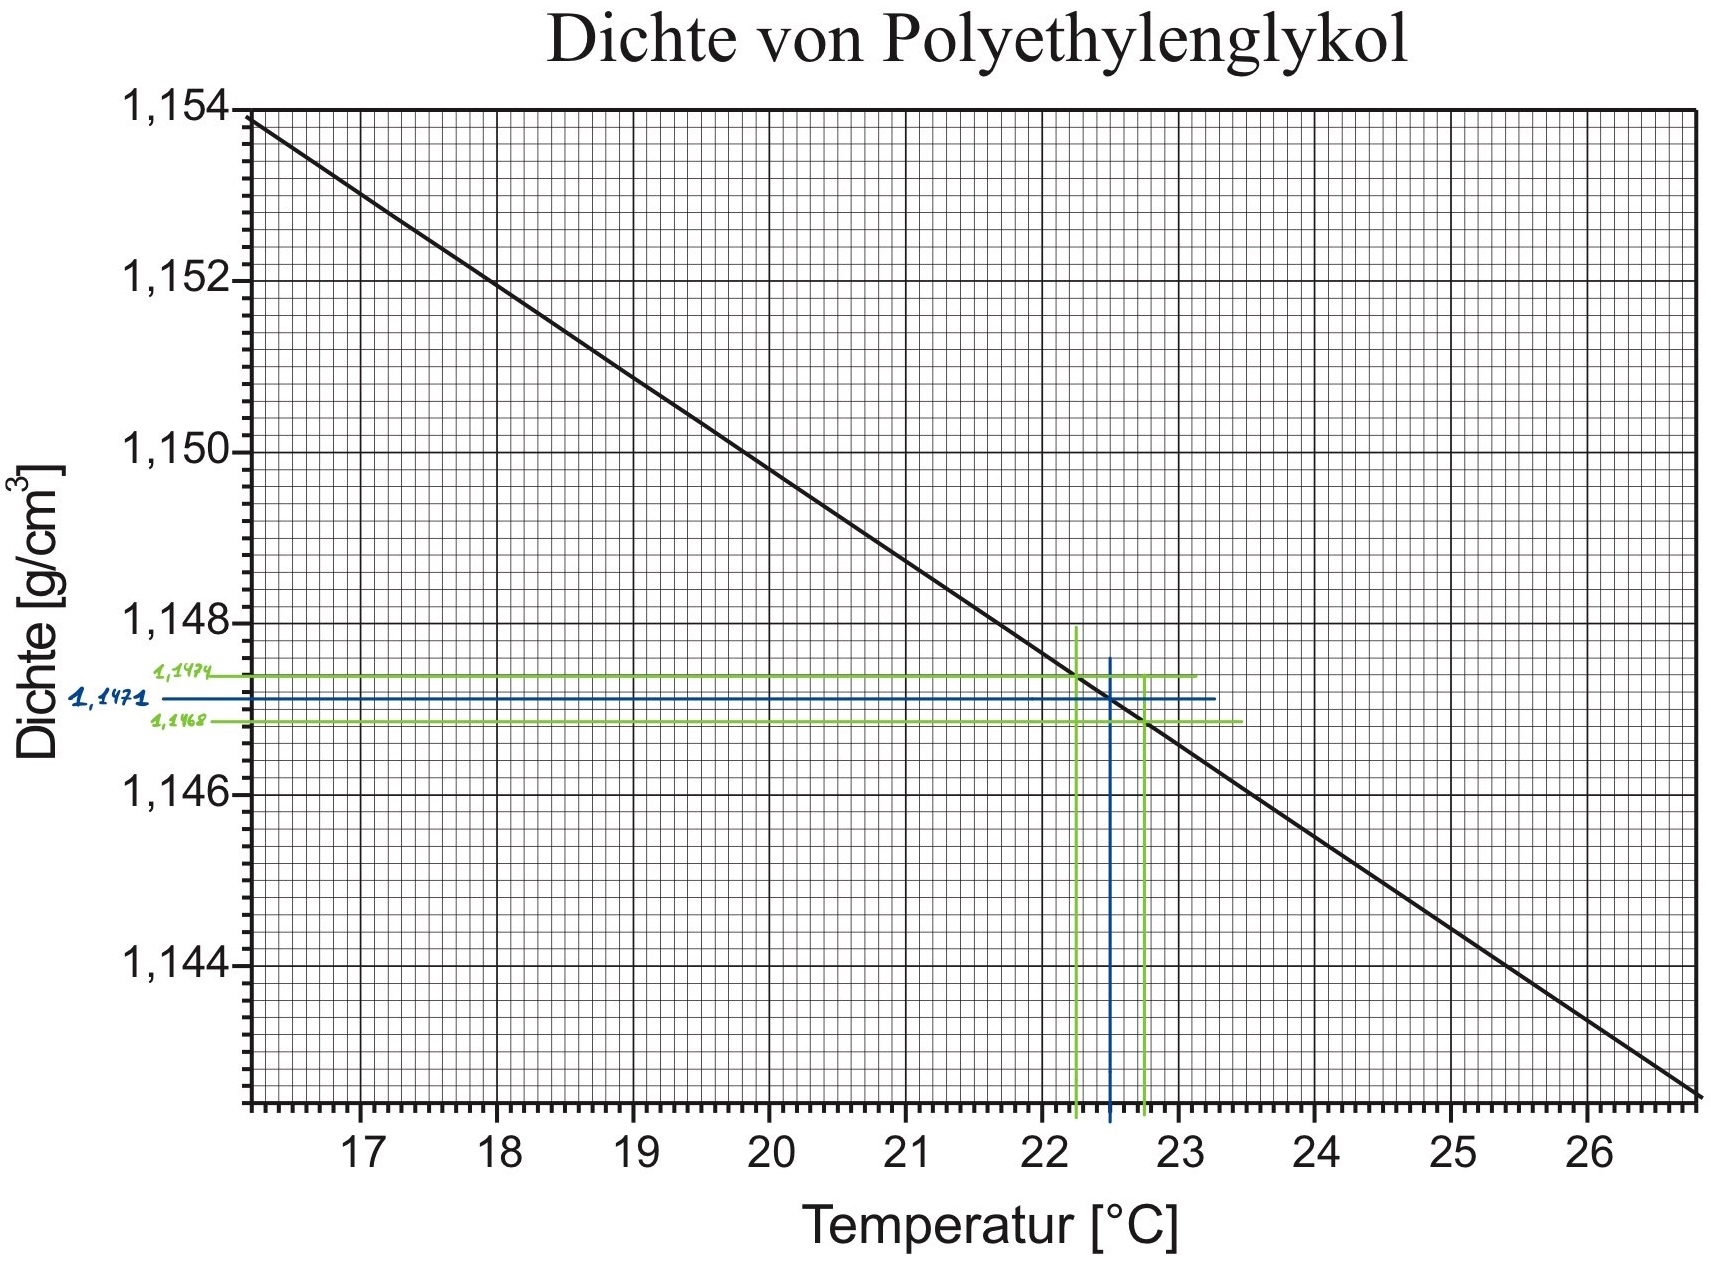
\includegraphics{graphics/212_-_Zahigkeit-8.jpg}}
    \caption{Bestimmung der Dichte in Abhängigkeit der Temperatur [Quelle Diagramm: PAP2.1 Skript, S.16, Stand: 27.02.2024]}
    \label{fig:Dichte_f}
\end{figure}

\phantom{.}

Damit können wir nun die Viskosität mittels Gleichung \ref{eq:visk_stokes} bestimmen:

\begin{equation}
    \begin{split}
        \eta_s &= \frac{2}{9} \ g \ \frac{(\rho_k - \rho_f)}{\gamma} \\
        \Delta \eta_s &= \eta \sqrt{\left( \frac{\Delta (\rho_k - \rho_f)}{(\rho_k - \rho_f)} \right)^2 + \left( \frac{\Delta \gamma}{\gamma} \right)^2} \\ \\
        &\Rightarrow \eta_s = (0,233 \pm 0,017) \text{Pa} \cdot \text{s}
    \end{split}
\end{equation}

Wir möchten mit dem nun bestimmten Wert der Viskosität rückwärtig die nach Gleichung \ref{eq:visk_stokes}
theoretisch erwarteten laminaren Sinkgeschwindigkeiten $v_{lam}$ bestimmen. Wir berechnen also für alle neun Radien die Werte:

\begin{equation}
    \begin{split}
        v_{lam} &= \frac{2}{9} \ g \ \frac{(\rho_k - \rho_f)}{\eta} \ r^2 \\
        \Delta v_{lam} &= v_{lam} \sqrt{\left( \frac{\Delta (\rho_k - \rho_f)}{(\rho_k - \rho_f)} \right)^2 + \left( \frac{\Delta \eta}{\eta} \right)^2 + \left( 2 \frac{\Delta r}{r} \right)^2}
    \end{split}
\end{equation}

Diese Werte vergleichen wir über Signifikanztests mit den korrigierten Geschwindigkeiten und tragen die Ergebnisse in Tabelle \ref{tab:v_lam} ein.

\phantom{.}

\begin{table}[!h]
    \centering
    %\resizebox{\textwidth}{!}{
    \begin{tabular}{cccc}
        \hline
        \textbf{Kugel} & $\bm{v_{lam}}$ [mm/s] & $\bm{v_{korr}}$ [mm/s] & $\bm{\sigma_{lk}}$  \\ \hline
        1 & $0,56 \pm 0,06$ & $0,69 \pm 0,07$ & $1,5$     \\
        2 & $2,23 \pm 0,22$ & $2,24 \pm 0,26$ & $0,027$     \\
        3 & $5,0 \pm 0,5$   & $5,3 \pm 0,6$ & $0,4$     \\
        4 & $8,9 \pm 0,9$   & $8,7 \pm 0,5$ & $0,25$     \\
        5 & $13,9 \pm 1,3$  & $15,0 \pm 0,9$ & $0,6$     \\
        6 & $20,1 \pm 1,9$  & $19,1 \pm 0,6$ & $0,5$     \\
        7 & $27,3 \pm 2,6$  & $26,6 \pm 1,1$ & $0,24$     \\
        8 & $36 \pm 3$      & $33,4 \pm 1,3$ & $0,6$     \\
        9 & $45 \pm 4$      & $41,7 \pm 1,8$ & $0,7$     \\ \hline
    \end{tabular}%}
    \caption{Theoretische Fallgeschwindigkeiten}
    \label{tab:v_lam}
\end{table}

\phantom{.}

Alle Signifikanztests liegen hierbei innerhalb insignifikanter Abweichungen. Nur der Vergleich bei den Werten der kleinsten Kugel ist mit einer Abweichung von 1,5 etwas erhöht, aber immer noch unterhalb der $3\sigma$-Grenze.

Nun berechnen wir noch das Verhältnis der gemessenen Geschwindigkeiten $v$ zu $v_{lam}$ sowie die Reynoldszahl $Re$ für jede Kugel. Für Letzteres verwenden wir Gleichung \ref{eq:Reynolds_L}, wobei wir $\rho_f$ und die gemessenen Geschwindigkeiten $v$ einsetzen. Wir tragen alle Ergebnisse in Tabelle \ref{tab:v_lam&Re} ein, wobei sich die letzten beiden Fehler folgendermaßen ergeben:

\begin{equation}
    \Delta \left( \frac{v}{v_{lam}} \right) =  \frac{v}{v_{lam}} \sqrt{\left( \frac{\Delta v}{v} \right)^2 + \left( \frac{\Delta v_{lam}}{v_{lam}} \right)^2}
\end{equation}

\begin{equation}
    \Delta Re = Re \sqrt{\left( \frac{\Delta v}{v} \right)^2 + \left( \frac{\Delta \rho_f}{\rho_f} \right)^2 + \left( \frac{\Delta d}{d} \right)^2 + \left( \frac{\Delta \eta}{\eta} \right)^2}
\end{equation}

Die Ergebnisse werden gegeneinander in ein Diagramm eingetragen, Abbildung \ref{fig:StokesReynold}, und wir schätzen daran die kritische Reynoldszahl ab. Diese ist dort, wo der Graph einen sichtbareren Knick bekommt. Wir schätzen somit den Wert:

\begin{equation}
    Re_{krit} = 0,48 \pm 0,28.
\end{equation}

Der Fehler wurde aus dem Abstand zu den nächsten Reynoldszahlen abgeschätzt. Bedauerlicherweise war der Knick im Diagramm nicht allzu gut zu erkennen, der gewählte Punkt wirkte jedoch am sinnvollsten. Vergleicht man den bestimmten Wert mit dem theoretisch erwarteten Wert von 1 so ergibt sich eine Abweichung von $\sigma_{Re} = 1,9$. Dies ist zwar etwas erhöht aber generell immer noch im insignifikanten Bereich. 

\phantom{.}

\begin{table}[!h]
    \centering
    %\resizebox{\textwidth}{!}{
    \begin{tabular}{cccc}
        \hline
        \textbf{Kugel} & $\bm{v_{lam}}$ [mm/s] & $\bm{v/v_{lam}}$ & $\bm{Re}$  \\ \hline
        1 & $0,56 \pm 0,06$ & $1,21 \pm 0,18$ & $0,0033 \pm 0,0004$     \\
        2 & $2,23 \pm 0,22$ & $0,95 \pm 0,15$ & $0,0209 \pm 0,0029$     \\
        3 & $5,0 \pm 0,5$   & $0,98 \pm 0,14$ & $0,073 \pm 0,009$     \\
        4 & $8,9 \pm 0,9$   & $0,87 \pm 0,10$ & $0,154 \pm 0,014$     \\
        5 & $13,9 \pm 1,3$  & $0,94 \pm 0,11$ & $0,32 \pm 0,03$     \\
        6 & $20,1 \pm 1,9$  & $0,82 \pm 0,08$ & $0,48 \pm 0,04$     \\
        7 & $27,3 \pm 2,6$  & $0,82 \pm 0,09$ & $0,77 \pm 0,06$     \\
        8 & $36 \pm 3$      & $0,77 \pm 0,08$ & $1,08 \pm 0,09$     \\
        9 & $45 \pm 4$      & $0,74 \pm 0,08$ & $1,48 \pm 0,12$     \\ \hline
    \end{tabular}%}
    \caption{Verhältnis der Geschwindigkeiten \& Reynoldszahlen}
    \label{tab:v_lam&Re}
\end{table}

\phantom{.}

\begin{figure}[!h]
    \centering
    \resizebox{0.9\textwidth}{!}{
    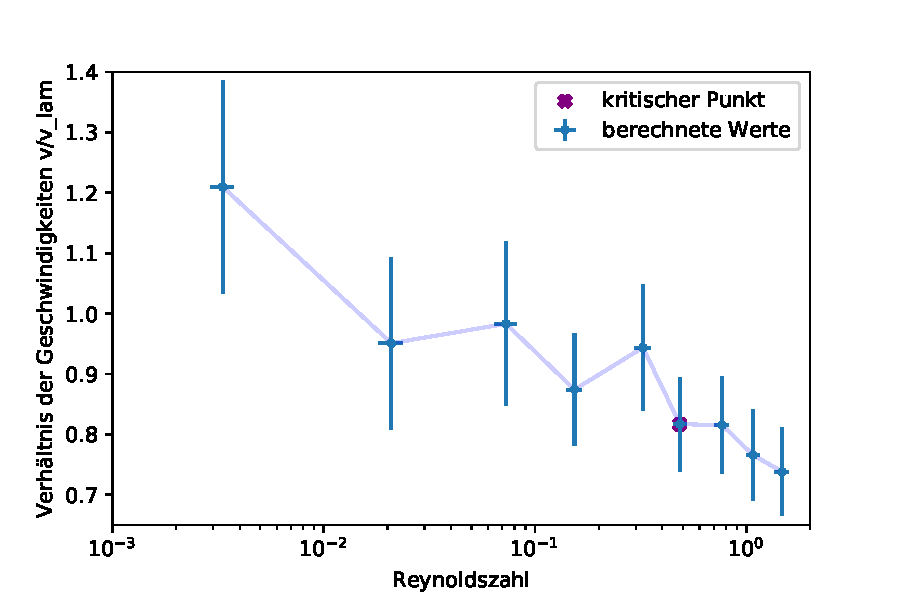
\includegraphics{graphics/plots/Reynolds_Stokes.pdf}}
    \caption{Verhältnis der Geschwindigkeiten und Reynoldszahlen - Bestimmung der kritischen Reynoldszahl}
    \label{fig:StokesReynold}
\end{figure}

\clearpage
\newpage
\subsection{Bestimmung der Viskosität nach Hagen-Poiseuille}

Für den zweiten Weg die Viskosität zu bestimmen plotten wir die gemessenen Werte des ausgeströmten Volumen aus Tabelle 2 des Messprotokolls als Funktion der Zeit. An die Messwerte fitten wir eine Gerade, dargestellt in Abbildung \ref{fig:FitHP}. Der Fit berechnet den Gradienten der Steigung, welcher dem Volumenstrom entspricht:

\begin{equation}
    \frac{dV}{dt} = (3,26 \pm 0,06) \cdot 10^{-8} \ \frac{\text{m}^3}{\text{s}}
\end{equation}

\phantom{.}

\begin{figure}[!h]
    \centering
    \resizebox{0.9\textwidth}{!}{
    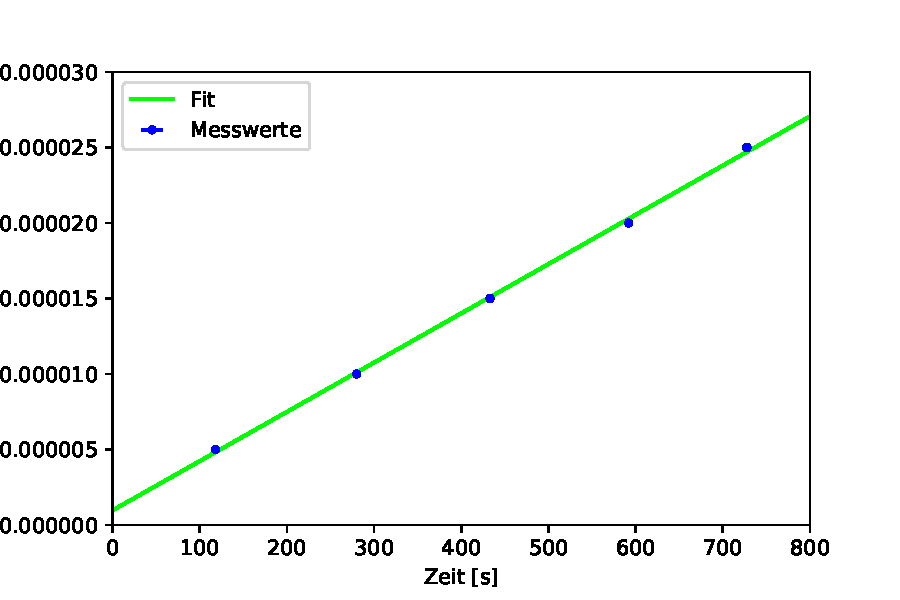
\includegraphics{graphics/plots/Fit_HP.pdf}}
    \caption{Linearer Fit für den Volumenstrom}
    \label{fig:FitHP}
\end{figure}

\phantom{.}

Für die Viskosität benötigen wir nun noch vier weitere Werte:

Den Mittelwert der Höhe, der aus der Anfangshöhe $h_A$ und der Endhöhe $h_E$ berechnet wird:

\begin{equation}
    \begin{split}
        h_m &= \frac{1}{2} (h_A + h_E), \ \ \ \ \ \Delta h_m = \frac{1}{2} \sqrt{(\Delta h_A)^2 + (\Delta h_E)^2} \\
        &\Rightarrow h_m = (0,5020 \pm 0,0007) \text{m}        
    \end{split}
\end{equation}

Die Druckdifferenz $dp$ von den Enden der Kapillare. Da vom Behälter aus Luftdruck sowie Schweredruck des Fluids und vom anderen Ende nur der Luftdruck wirkt, ist die Differenz einfach der Schweredruck des Polyethylenglykols. Dieser berechnet sich folgendermaßen:

\begin{equation}
    \begin{split}
        dp &= \rho_f g h_m, \ \ \ \ \ \Delta dp = dp \sqrt{\left( \frac{\Delta \rho_f}{\rho_f} \right)^2 + \left( \frac{\Delta h_m}{h_m} \right)^2} \\
        &\Rightarrow dp = (5647 \pm 8) \text{Pa}
    \end{split}
\end{equation}

Des Weiteren benötigen wir noch die Länge $L_{kap}$ sowie den Radius $R_{kap}$ des Kapillars. Diese entnehmen wir dem Skript:

\begin{equation}
    \begin{split}
        L_{kap} &= (1000 \pm 5) \cdot 10^{-4} \text{m} \\
        R_{kap} &= (750 \pm 5) \cdot 10^{-6} \text{m}
    \end{split} 
\end{equation}

Damit haben wir alles um nach Gleichung \ref{eq:HagPois} die Viskosität zu bestimmen. Der Fehler wird mit

\begin{equation}
    \Delta \eta_{HP} = \eta_{HP} \sqrt{\left( \frac{\Delta dp}{dp} \right)^2 + \left( \frac{\Delta \frac{dV}{dt}}{\frac{dV}{dt}} \right)^2 + \left( \frac{\Delta L_{kap}}{L_{kap}} \right)^2 + \left( 4 \frac{\Delta R_{kap}}{R_{kap}} \right)^2}
\end{equation}

berechnet und somit erhalten wir:

\begin{equation}
    \eta_{HP} = (0,215 \pm 0,007) \text{Pa} \cdot \text{s}.
\end{equation}

Verglichen mit der über Stokes berechneten Viskosität erhalten wir eine Abweichung von $\sigma_{\eta} = 0,98$, was nicht signifikant ist.

Zuletzt möchten wir auch hier die Reynoldszahl berechnen. Dazu muss die mittlere Strömungsgeschwindigkeit $v_{kap}$ bestimmt werden, welche sich aus dem Volumenstrom bestimmen lässt, indem man durch die Querschnittsfläche $A = \pi R_{kap}^2$ teilt:

\begin{equation}
    \begin{split}
        v_{kap} &= \frac{\frac{dV}{dt}}{A} = \frac{\frac{dV}{dt}}{\pi R_{kap}^2} \\
        \Delta v_{kap} &= v_{kap} \sqrt{\left( \frac{\Delta \frac{dV}{dt}}{\frac{dV}{dt}} \right)^2 + \left( 2 \frac{\Delta R_{kap}}{R_{kap}} \right)^2} \\ \\
        &\Rightarrow v_{kap} = (18,5 \pm 0,4) \frac{\text{mm}}{\text{s}}
    \end{split}
\end{equation}

Damit berechnen wir die Reynoldszahl nach Gleichung \ref{eq:Reynolds_L}, wobei die charakteristische Länge $L$ hier der Durchmesser der Kapillare ist:

\begin{equation}
    \begin{split}
        Re_{HP} &= \frac{2 \rho_f v_{kap} R_{kap}}{\eta_{HP}} \\
        \Delta Re_{HP} &= Re_{HP} \sqrt{\left( \frac{\Delta \rho_f}{\rho_f} \right)^2 + \left( \frac{\Delta v_{kap}}{v_{kap}} \right)^2 + \left( \frac{\Delta R_{kap}}{R_{kap}} \right)^2 + \left( \frac{\Delta \eta_{HP}}{\eta_{HP}} \right)^2} \\ \\
        &\Rightarrow Re_{HP} = 0,148 \pm 0,006
    \end{split}
\end{equation}

Dieser Wert liegt deutlich unterhalb der experimentell festgelegten kritischen Reynoldszahl von 2300 für Rohrströmungen. Somit ist bestätigt, dass es sich bei unserer Strömung wirklich um eine laminare Strömung handelte.

\newpage
%---------------PRÄSENTATION DER ENDERGEBNISSE---------------
\section{Zusammenfassung der Endergebnisse}

In diesem Versuch wurde auf zwei verschiedene Wege die Viskosität von Polyethylenglykol bestimmt. Beim ersten Teil berechneten wir über Fallzeitmessungen im Kugelviskosimeter nach Stokes den Wert

\begin{equation}
    \eta_s = (0,233 \pm 0,017) \text{Pa} \cdot \text{s}.
\end{equation}

Hierzu berechneten wir zunächst die Ladenburg'sche Korrektur für die gemessenen Fallzeiten $v_{korr}$ und trugen die so bestimmten Fallgeschwindigkeiten gegen den quadrierten Kugelradius in ein Diagramm ein, um aus der Steigung des linearen Teils die Viskosität zu bestimmen. 

Im zweiten Teil bestimmten wir den Volumenstrom einer laminaren Strömung des Fluids und berechneten nach dem Gesetz von Hagen-Poiseuille den Wert

\begin{equation}
    \eta_{HP} = (0,215 \pm 0,007) \text{Pa} \cdot \text{s}.
\end{equation}

Diese beiden Werte weisen eine insignifikante Abweichung von $\sigma_{\eta} = 0,98$ voneinander auf. Dies zeigt, dass bis auf kleinere Messungenauigkeiten keine größeren grundlegenden oder systematischen Fehler bei den zwei verschiedenen Versuchsteilen vorlagen.

Des Weiteren bestimmten wir im ersten Teil zunächst aus der Viskosität die theoretisch erwarteten Fallgeschwindigkeiten $v_{lam}$ sowie die Reynoldszahl für jeden Kugelradius. Bei Vergleich der theoretischen Geschwindigkeiten $v_{lam}$ mit den zuvor bestimmten korrigierten Messwerten $v_{korr}$ wurden keine signifikanten Abweichungen festgestellt. Allein die Werte der kleinsten Kugel mit 1mm Durchmesser wiesen mit einer Abweichung von 1,5 einen leicht erhöhten Wert auf. Abschließend bestimmten wir mithilfe eines Diagramms, in dem das Verhältnis der gemessenen zu den theoretischen Geschwindigkeiten gegen die bestimmten Reynoldszahlen aufgetragen wurde, einen ungefähren Wert für die kritische Reynoldszahl der Bewegung von Kugeln durch die Flüssigkeit: 

\begin{equation}
    Re_{krit} = 0,48 \pm 0,28
\end{equation}

Im Vergleich zum theoretisch erwarteten Wert von 1 liegt hier eine Abweichung von $\sigma_{Re} = 1,9$ vor. 

Im zweiten Teil berechneten wir noch die Reynoldszahl der vermessenen Strömung mithilfe der zuvor bestimmten mittleren Strömungsgeschwindigkeit $v_{kap}$ in der Kapillare:

\begin{equation}
    Re_{HP} = 0,148 \pm 0,006.
\end{equation}

Dieser Wert liegt unterhalb der kritischen Reynoldszahl von 2300 für Rohrströmungen und bestätigt somit, dass es sich um eine laminare Rohrströmung handelte. 

\newpage
%---------------ZUSAMMENFASSUNG UND DISKUSSION---------------
\section{Diskussion}

Allgemein kann man sagen, dass der Versuch größtenteils gute Ergebnisse geliefert hat. Die Plots der direkt gemessenen sowie der korrigierten Geschwindigkeiten in Teil Eins ergaben Sinn und auch der lineare Fit sowie die darauf folgende Berechnung von $\eta_s$ haben gut geklappt. Weiterführend erscheinen die berechneten theoretischen Geschwindigkeiten $v_{lam}$ sowie die bestimmten Reynoldszahlen jeweils recht sinnvoll und auch die Signifikanztests der $v_{lam}$ wiesen keine signifikanten Abweichungen auf. Der leicht erhöhte Wert beim Signifikanztest der kleinsten Kugel lässt sich vermutlich auf kleinere Messungenauigkeiten zurückführen. Die kleinsten Kugeln waren mit großem Abstand am langsamsten und zudem durch ihre sehr kleinen Ausmaße häufig schwer genau zu erkennen. Optische Verzerrungen am Glas und im Fluid sowie generelle Ungenauigkeiten beim manuellen Zeitstoppen können hier Einfluss auf die Messungen gehabt haben. Zudem kommt, dass die kleinen Kugeln häufig schwerer in das Fallviskosimeter einzuführen waren, da sie fast immer an der Pinzette hängen oder an der Oberfläche liegen blieben. Somit war es schwierig, diese mit gleichem Abstand vom Rohrrand und gleichen Anfangsbedingungen fallen zu lassen. Dennoch ist die berechnete Abweichung von 1,5 nicht signifikant und bedeutet, dass keine größeren Ungenauigkeiten oder gröbere, systematische Fehler aufgetreten sind. 

Jedoch verlief die anschließende Bestimmung der kritischen Reynoldszahl etwas holprig, was vor allem dem Fakt geschuldet ist, dass unser Plot der Geschwindigkeitsverhältnisse zu den Reynoldszahlen nicht den erwarteten Verlauf aufzeigte. Vor allem die großen Sprünge nach oben und unten für die ersten paar Reynoldszahlen sind hier auffällig. Diese kommen davon, dass unsere theoretisch berechneten Werte $v_{lam}$, die alle ziemlich genau auf der Fitgeraden liegen, bei den ersten paar Werten teils kleiner und teils größer als die aus den Messungen berechneten Geschwindigkeiten $v$ sind. Grund ist, dass unsere ersten Werte etwas um die Fitgerade streuen, was höchstwahrscheinlich Resultate der bereits genannten Messungenauigkeiten bei den kleineren Kugeln sein, die sich hier deutlicher gezeigt haben. Somit war die Bestimmung der kritischen Reynoldszahl erschwert und konnte nur anhand der letzten Paar Punkte, die einen geraderen Verlauf zeigten, abgeschätzt werden. Dies erklärt auch die leicht erhöhte Abweichung vom erwarteten Wert von 1,9.

Dahingegen verlief der zweite Versuchsteil wieder praktisch einwandfrei. Der Fit und die weiteren Berechnungen lieferten zuverlässige Ergebnisse und die berechnete Viskosität passt sehr gut zu der des ersten Versuchsteils, was eine aussagekräftige Bestätigung der im Versuch untersuchten Theorien darstellt. Auch klappte hier die Berechnung der Reynoldszahl gut und lieferte ein erwartetes, zur Theorie passendes Ergebnis. Allgemein lässt sich hier nur anmerken, dass die Zeitmessung des Volumenstroms in der hier durchgeführten Form kleinere Messfehler zulässt. Ein Aspekt wäre hier die Verzögerung vom Moment, ab dem der Tropfen aus der Kapillare fällt, bis zu dem, wenn er im Messbecher landet. Auch treten hier allgemein wieder optische Verzerrungen bei der Ablesung des Volumens durch Glas und Fluid auf sowie die üblichen Reaktionszeitfehler aufgrund der manuellen Zeitstoppung.

Mögliche Verbesserungen des Versuchsaufbaus wären im ersten Teil eine Form von kontrolliertem Einlass der Kugeln ins Fallviskosimeter, sodass eine möglichst zentrale Einführung mit gleichen Anfangsbedingungen für alle Kugeln ermöglicht wird. Auch wäre eine Digitalisierung der Zeitmessung mit beispielsweise Sensoren ein Weg, deutlich konsistentere Ergebnisse zu erzielen. Analog gilt dies auch für den zweiten Versuchsteil, wo eine digitale Zeit- und Volumenmessung nochmal genauere Ergebnisse erziehlen würde. 

Abschließend lässt sich also sagen, dass fast alle Teile des Versuchs aussagekräftige und plausible Ergebnisse lieferten, die zueinander passen und die Theorie nicht verletzen, wodurch die viskosen Eigenschaften von Polyethylenglykol aufschlussreich mit zwei unterschiedlichen Methoden untersucht werden konnten. 



\newpage
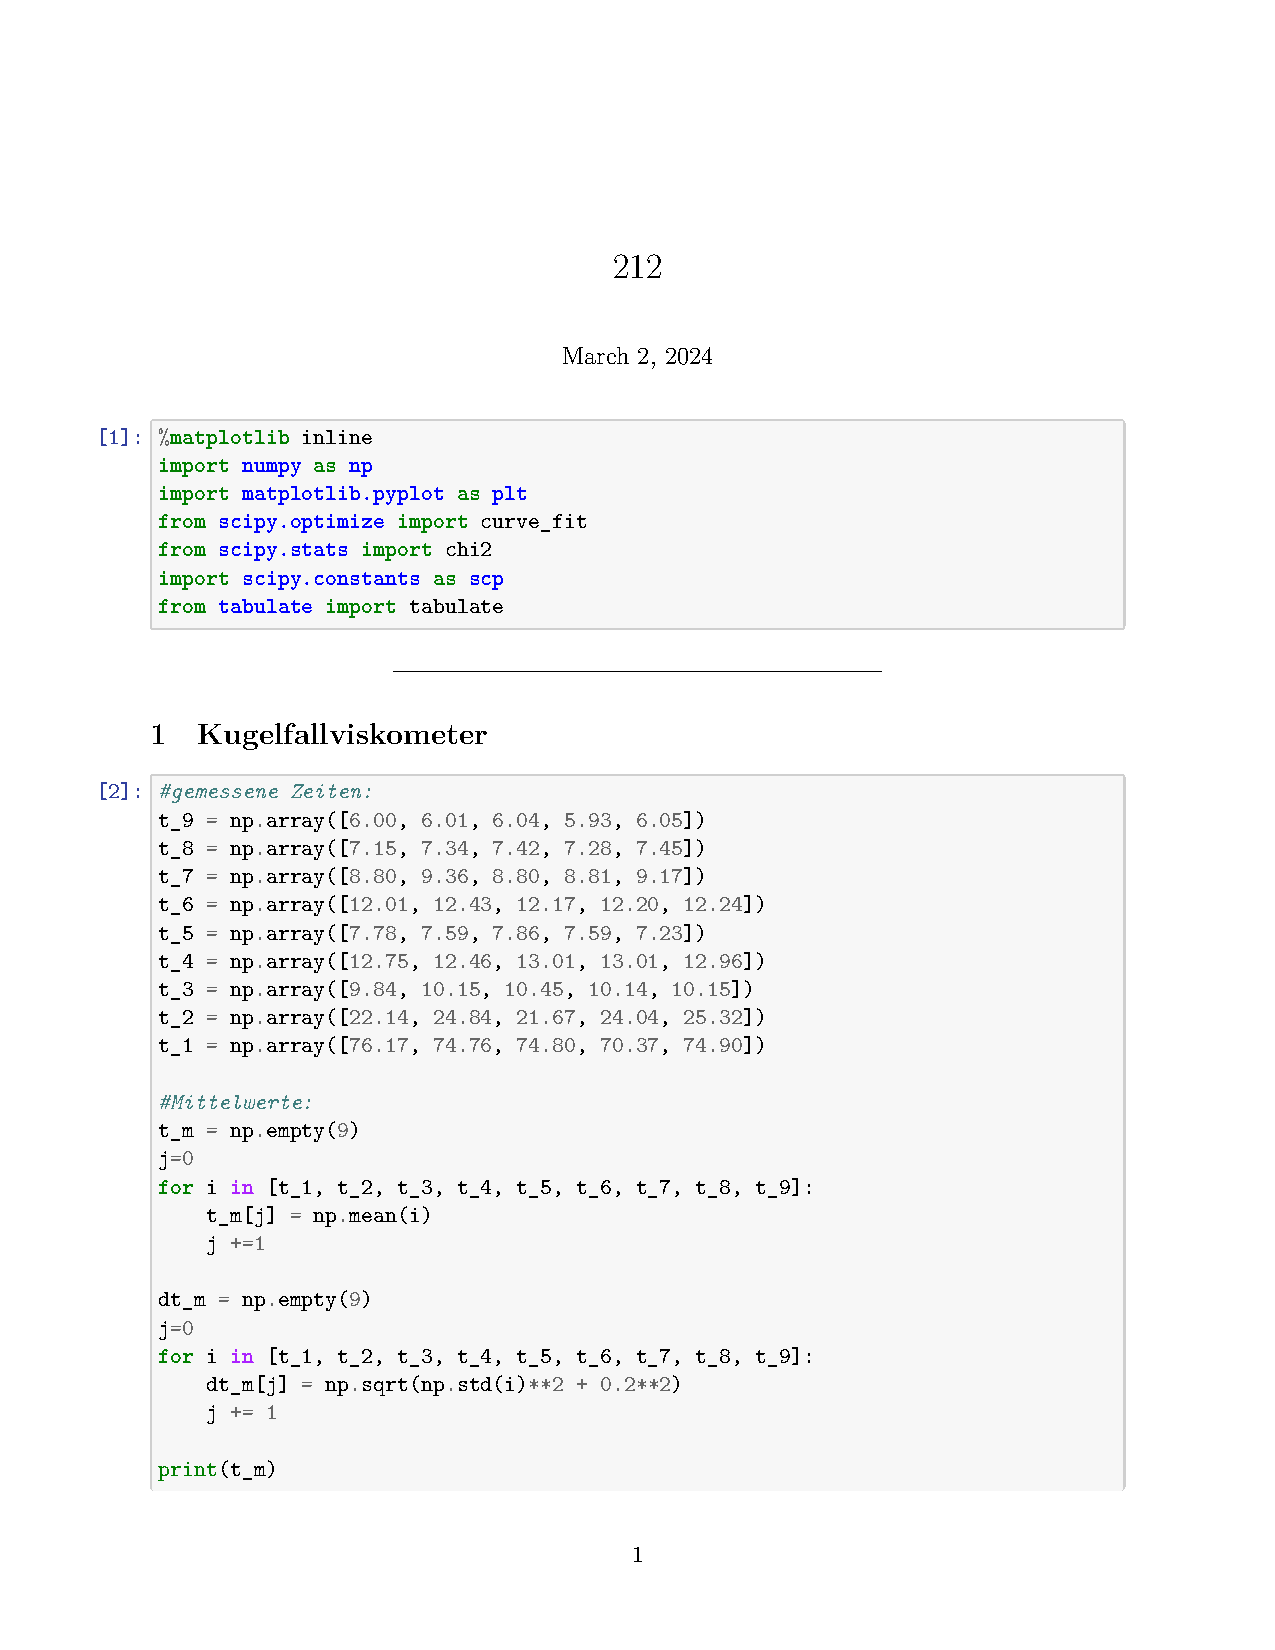
\includepdf[pages=-]{212.pdf}

\end{document}

